
\section{Binomial step selection evaluation}\label{app:binomial-eval}

The plots for the evaluation of binomial step size selection are provided in Figure~\ref{fig:empirical-evals-binomial}.  These are inferior to those shown in the main text for the uniform distribution in Figure~\ref{fig:empirical-evals}.

\begin{figure}
    \centering
    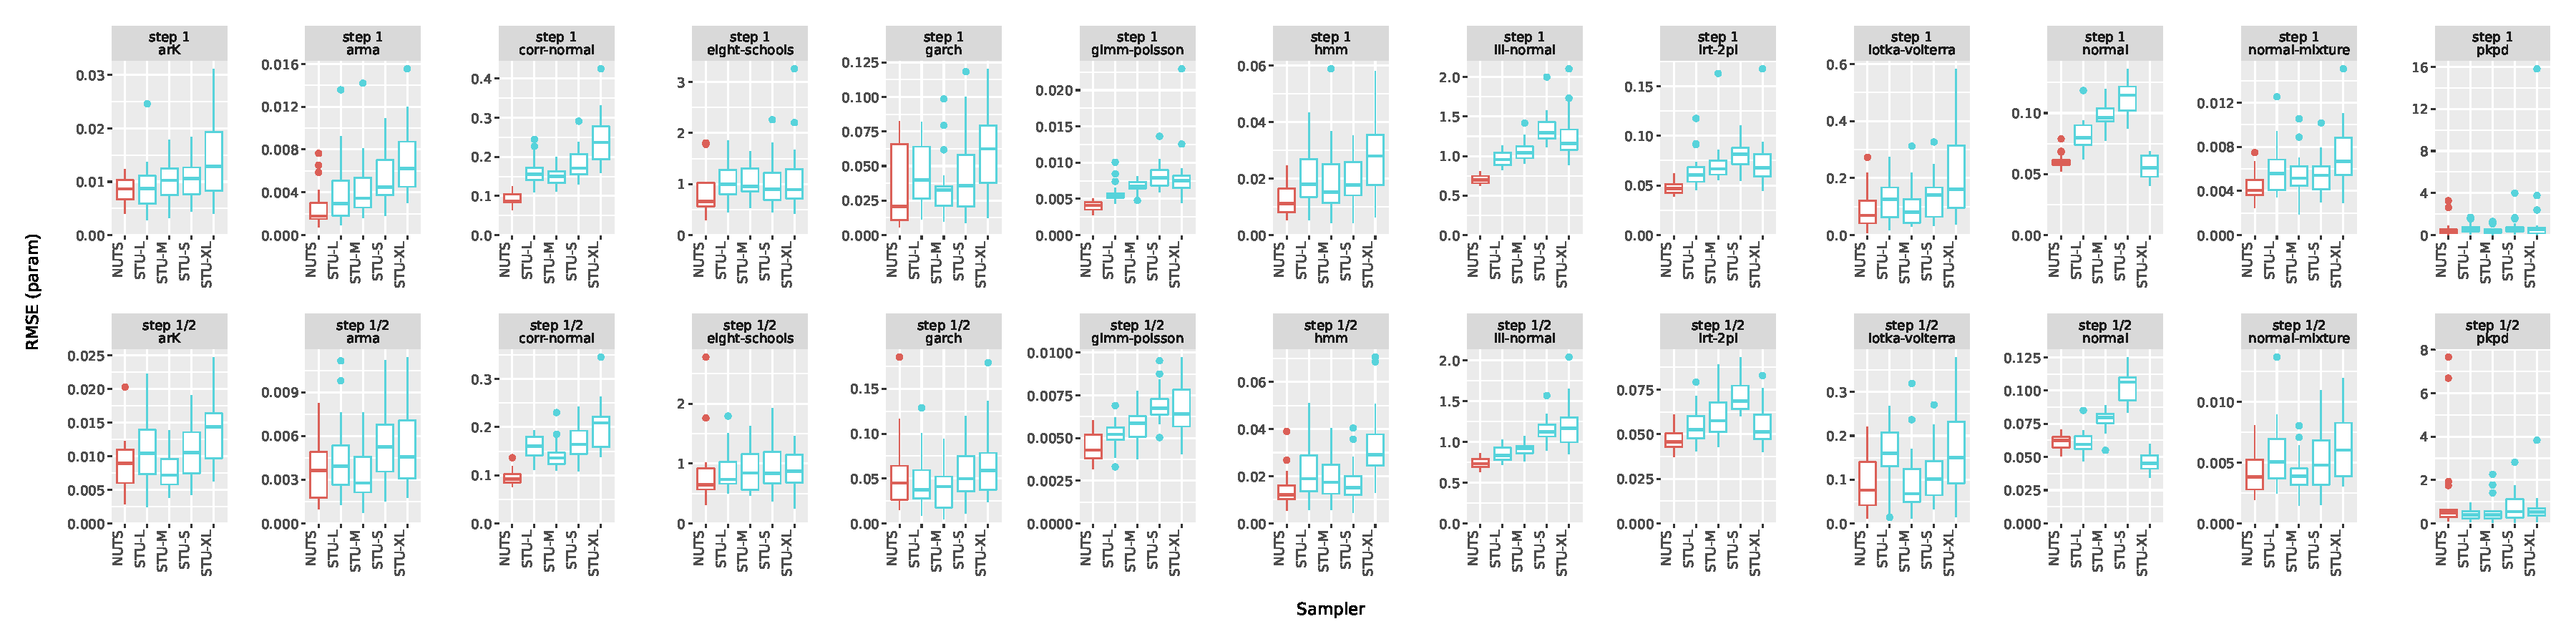
\includegraphics[width=\textwidth]{img/results/uniform/vs_nuts_RMSE_param.pdf}
    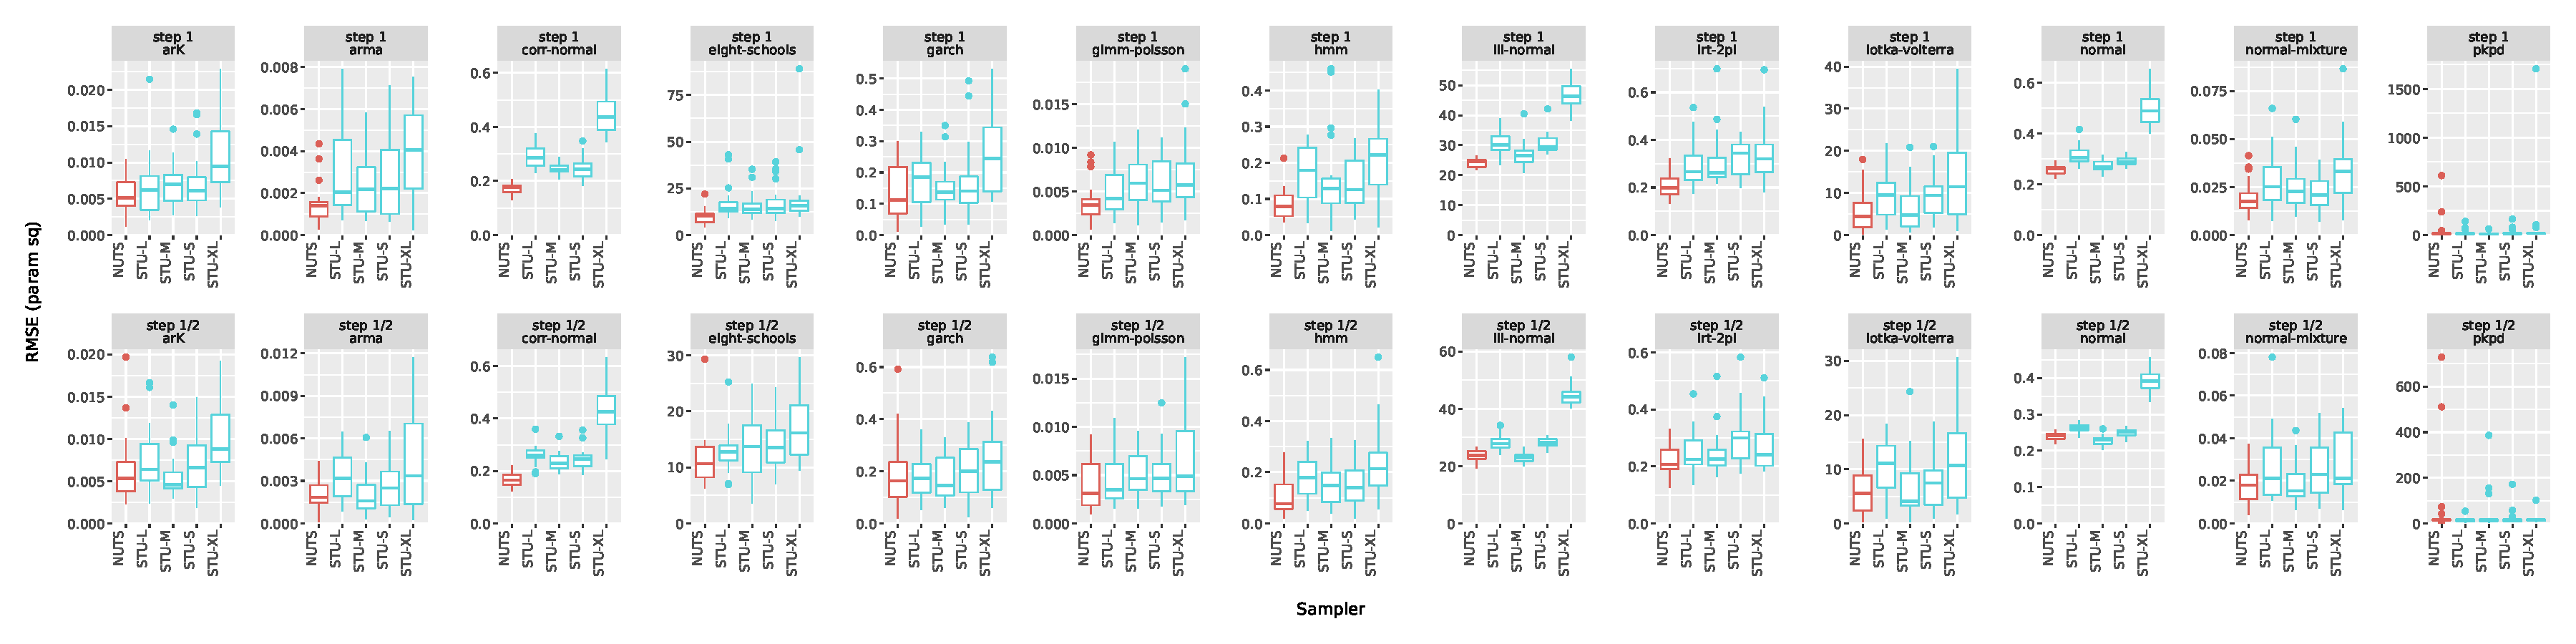
\includegraphics[width=\textwidth]{img/results/uniform/vs_nuts_RMSE_param_sq.pdf}
    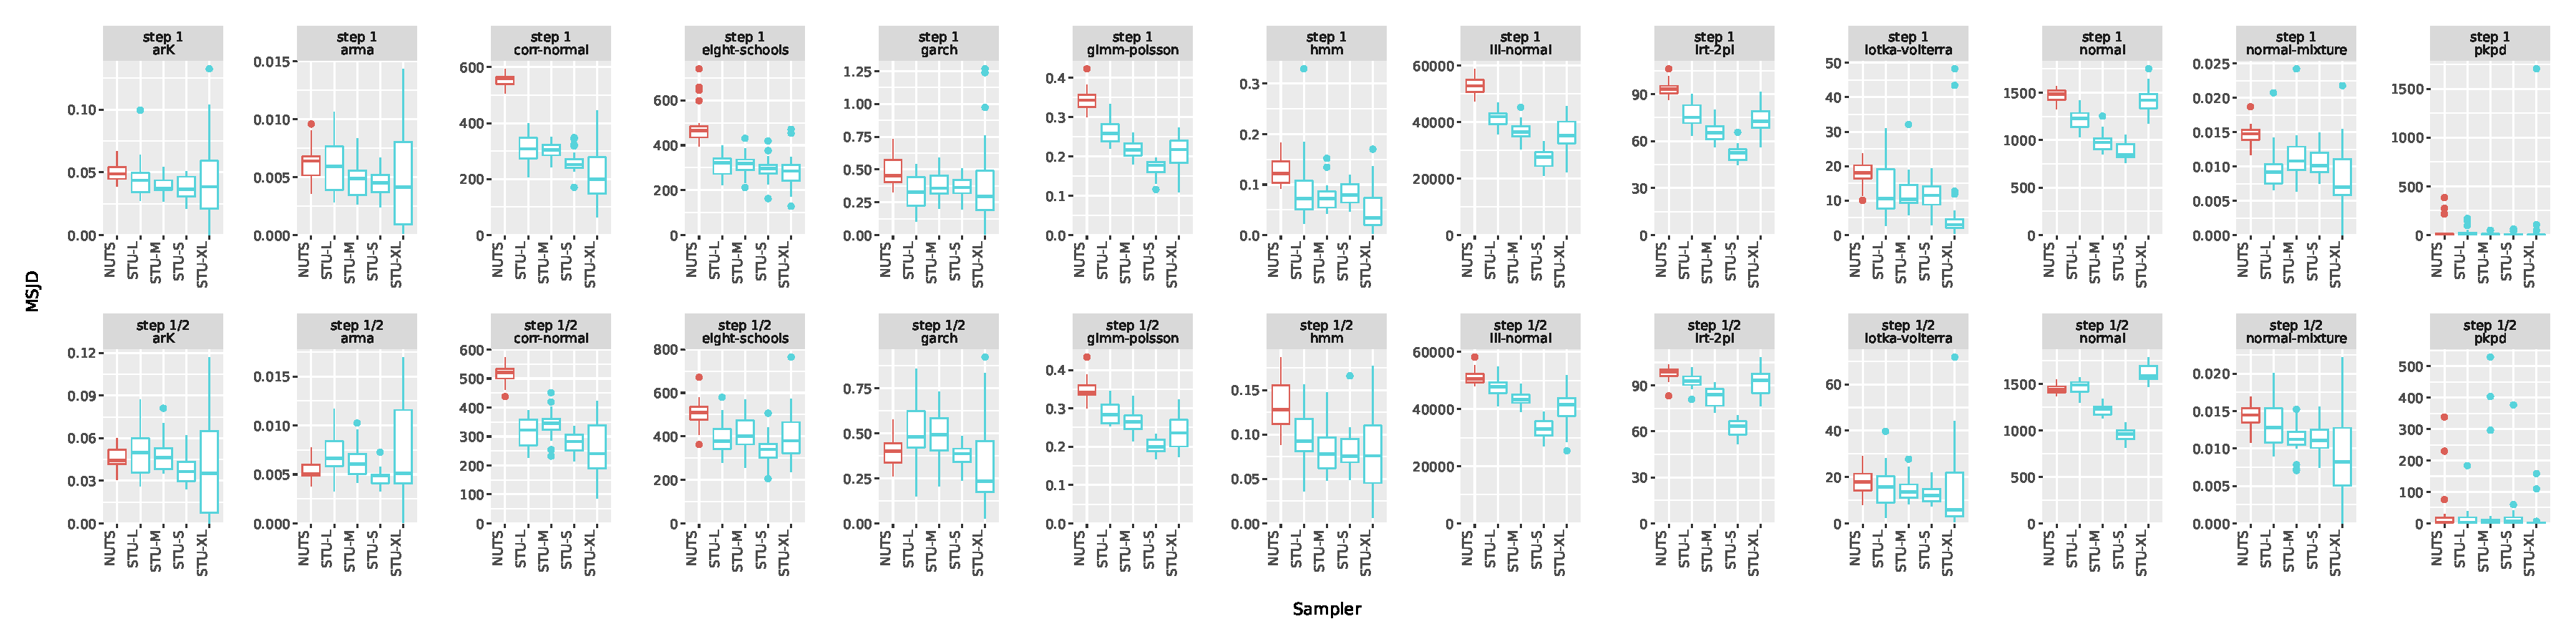
\includegraphics[width=\textwidth]{img/results/uniform/vs_nuts_MSJD.pdf}
    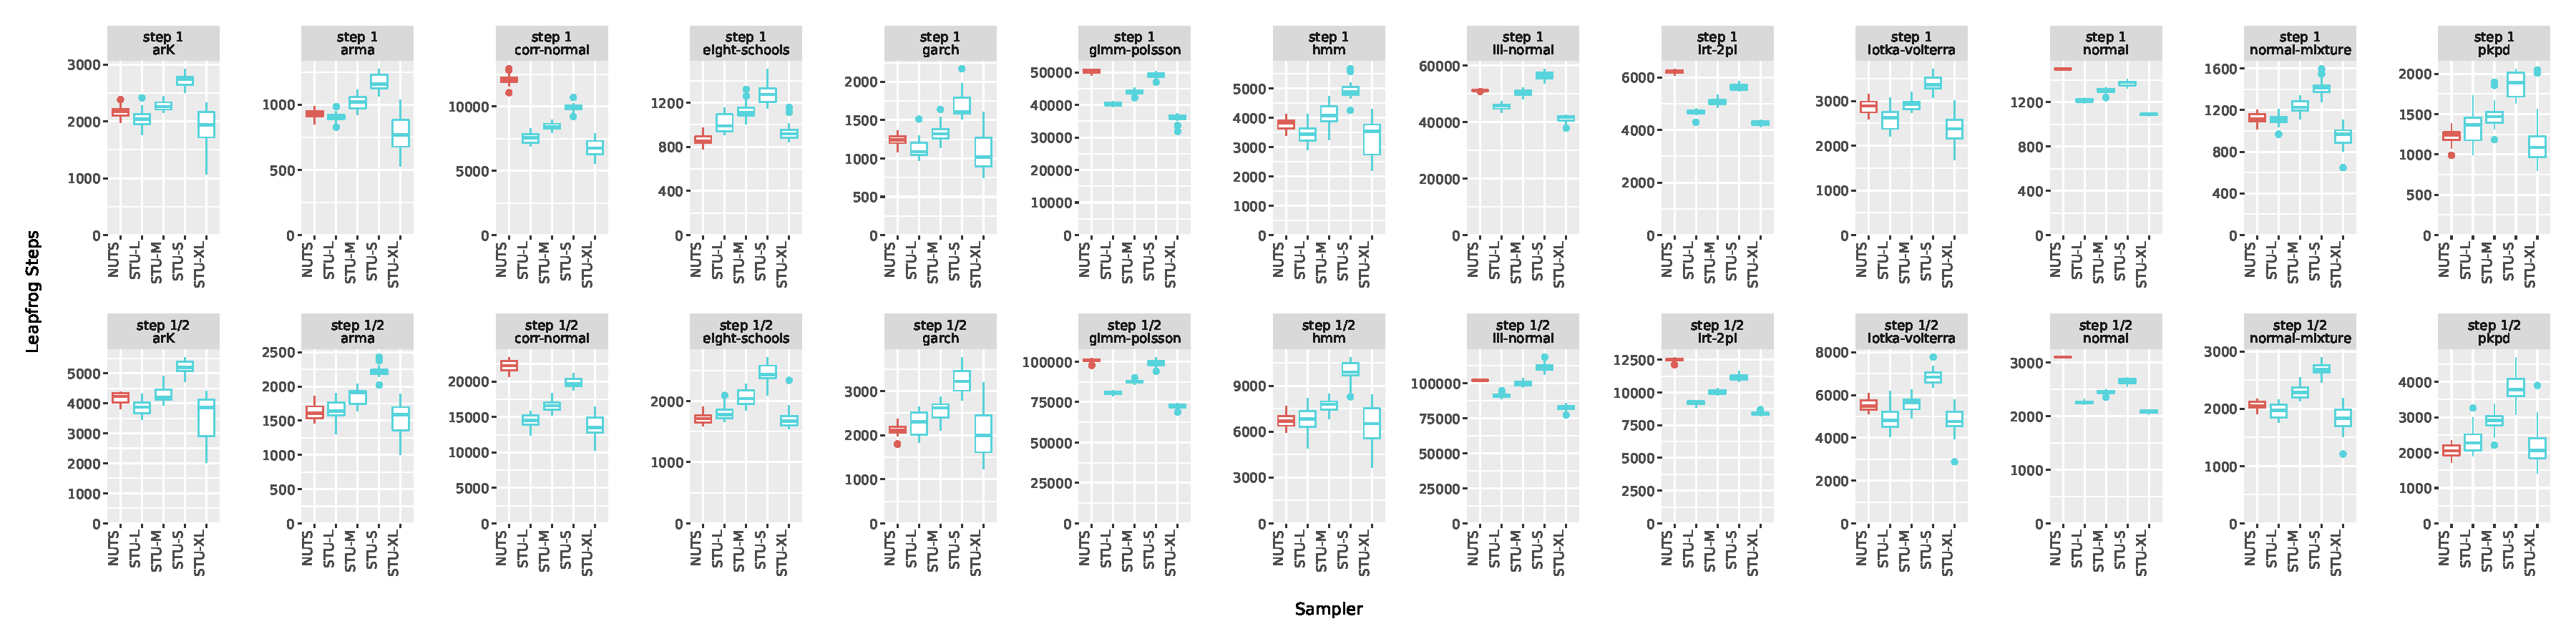
\includegraphics[width=\textwidth]{img/results/uniform/vs_nuts_Leapfrog_Steps.pdf}
    \caption{\it {\bfseries Empirical Evaluations vs.~NUTS}. Root mean square error of parameters, and parameters squared (lower is better), mean square jump distances (higher is better), and number of leapfrog steps (smaller is more efficient).  Each column is for a different model and the rows are for runs at NUTS default accepted step size (0.8 average Metropolis acceptance) and half of that rate, which is recommended for increased stability. The red result is NUTS and the blue results are for the self-tuning uniform sampler over intervals with small (S), medium (M), and large (L) expected values: $\textrm{uniform}(1, L)$, $\textrm{uniform}(\lfloor{L / 2}\rfloor, L)$, and $\textrm{uniform}(\lfloor{3L / 4}\rfloor, L)$.}
    \label{fig:empirical-evals-binomial}
\end{figure}